\documentclass[10pt,aspectratio=169]{beamer}

\mode<presentation>{
  \usetheme[
    progressbar=none,
    titleformat=regular,
    numbering=fraction
  ]{metropolis}
}

\usepackage{iftex}
\ifPDFTeX
  \usepackage[utf8]{inputenc}
  \usepackage[T1]{fontenc}
\else
  \usepackage{fontspec}
\fi
\usepackage[sfdefault,light,medium,lining]{FiraSans}
\usepackage{amsmath}
\usepackage{amssymb}
\usepackage{booktabs}
\usepackage{graphicx}
\usepackage{tcolorbox}
\usepackage[round,authoryear]{natbib}
\usepackage[capitalise,nameinlink]{cleveref}

\makeatletter
\setbeamertemplate{headline}{%
  \begin{beamercolorbox}[colsep=1.5pt]{upper separation line head}
  \end{beamercolorbox}
  \begin{beamercolorbox}{section in head/foot}
    \vskip1pt\insertnavigation{\paperwidth}\vskip1.5pt
  \end{beamercolorbox}%
  \begin{beamercolorbox}[colsep=1.5pt]{lower separation line head}
  \end{beamercolorbox}
}
\makeatother

\setbeamercolor{section in head/foot}{fg=normal text.bg,bg=structure.fg}
\setbeamercolor{background canvas}{bg=white}
\setbeamercovered{again covered={\opaqueness<1->{12}}}

\geometry{left=7mm,right=7mm}
\setbeamertemplate{footline}{%
  \begin{beamercolorbox}[wd=\textwidth,sep=1.1ex]{footline}%
    \usebeamerfont{page number in head/foot}%
    \usebeamertemplate*{frame footer}%
    \hfill\footnotesize\usebeamertemplate*{frame numbering}~
  \end{beamercolorbox}%
}

\definecolor{edf1}{rgb}{0,0.102,0.439}
\definecolor{edf2}{rgb}{0,0.357,0.733}
\definecolor{edf3}{rgb}{1,0.627,0.184}
\definecolor{edf4}{rgb}{0.996,0.345,0.082}
\definecolor{edf5}{RGB}{196,214,0}
\definecolor{edf6}{RGB}{80,158,47}
\definecolor{edf0}{RGB}{16,137,255}
\definecolor{sage}{RGB}{102,153,102}
\definecolor{bgcolor}{HTML}{ECF1FC}
\colorlet{colframe}{mDarkTeal}

\NewDocumentCommand{\ColorBox}{m m +m}{%
  \begin{tcolorbox}[
    colback=#1!15!white,
    colframe=colframe,
    coltitle=white,
    title={#2},
    fonttitle=\scshape,
    halign title=center,
    left=1mm,
    right=1mm,
    top=1mm,
    bottom=1mm,
    boxsep=4pt
  ]
    #3
  \end{tcolorbox}%
}

\NewDocumentCommand{\Figure}{m m m}{%
  \begin{figure}[!h]
    \centering
    \includegraphics[width=0.6\linewidth]{#1}
    \caption{#2}
    \label{#3}
  \end{figure}%
}

\NewDocumentCommand{\Forecasting}{}{%
  \Figure
    {Images/time-series/national-load-curves-forecast.pdf}
    {Individual electricity load}
    {fig:forecasting}%
}

\NewDocumentCommand{\PrintBibliography}{}{%
  \begin{frame}[allowframebreaks]{References}
    \footnotesize
    \bibliographystyle{plainnat}
    \bibliography{references}
  \end{frame}%
}

\NewDocumentCommand{\TimeSeriesPanel}{m m}{%
  \includegraphics[width=0.99\linewidth]{#1}\\[0.05cm]
  {\footnotesize #2\par}%
}

\NewDocumentCommand{\TimeSeriesOne}{}{%
  \begin{columns}[T,onlytextwidth]
    \begin{column}{0.49\textwidth}
      \centering
      \TimeSeriesPanel
        {Images/time-series/national-load-curves.pdf}
        {Aggregated load curve}
      \vspace{0.2cm}
      \TimeSeriesPanel
        {Images/time-series/ecg.pdf}
        {Heartbeat electrical activity}
    \end{column}
    \begin{column}{0.49\textwidth}
      \centering
      \TimeSeriesPanel
        {Images/time-series/traffic.pdf}
        {Road occupancy}
      \vspace{0.2cm}
      \TimeSeriesPanel
        {Images/time-series/solar.pdf}
        {Solar power generation}
    \end{column}
  \end{columns}%
}

\NewDocumentCommand{\TimeSeriesTwo}{}{%
  \begin{columns}[T,onlytextwidth]
    \begin{column}{0.49\textwidth}
      \centering
      \TimeSeriesPanel
        {Images/time-series/national-load-curves-forecast.pdf}
        {Forecasting}
      \vspace{0.2cm}
      \TimeSeriesPanel
        {Images/time-series/ecg-classification.pdf}
        {Classification}
    \end{column}
    \begin{column}{0.49\textwidth}
      \centering
      \TimeSeriesPanel
        {Images/time-series/traffic-imputation.pdf}
        {Imputation}
      \vspace{0.2cm}
      \TimeSeriesPanel
        {Images/time-series/solar-power-anomaly.pdf}
        {Anomaly detection}
    \end{column}
  \end{columns}%
}

% TeX reads \timeseries1 as the command \timeseries followed by the token 1.
% The dispatcher therefore supports both \timeseries1 and \timeseries{1}.
\ExplSyntaxOn
\NewDocumentCommand{\timeseries}{m}
  {
    \str_case:nnF {#1}
      {
        {1}{\TimeSeriesOne}
        {2}{\TimeSeriesTwo}
      }
      {
        \PackageError{csi-proposal}
          {Unknown~time-series~layout~'#1'}
          {Use~\string\timeseries1,~\string\timeseries2,~
           \string\timeseries{1},~or~\string\timeseries{2}.}
      }
  }
\ExplSyntaxOff

\title{Retrieval-Based Residual Adaptation}
\subtitle{A lightweight proposal for adapting pretrained time-series forecasters}
\author{Gaspard Berthelier}
\institute{EDF R\&D / Inria Sophia Antipolis}
\date{Neo Seminar -- \today}

\NewDocumentCommand{\TitleLogos}{}{%
  \hfill
  \begin{minipage}[t]{0.6\textwidth}
    \raggedleft
    
\includegraphics[height=0.6cm]{Logos/logo-edf.png}%
    \hspace{0.5cm}%
    
\includegraphics[height=0.6cm]{Logos/logo-inria.png}%
    \hspace{0.5cm}%
    
\includegraphics[height=0.6cm]{Logos/logo-uca.jpg}
  \end{minipage}%
}

\begin{document}

\begin{frame}[plain,noframenumbering]
  \vspace*{0.35cm}
  \TitleLogos

  \vspace{0.95cm}
  {\usebeamerfont{title}\inserttitle\par}

  \vspace{0.25cm}
  {\usebeamerfont{subtitle}\insertsubtitle\par}

  \vspace{0.45cm}
  {\color{edf4}\rule{\linewidth}{0.4pt}\par}

  \vspace{0.8cm}
  {\usebeamerfont{author}\insertauthor\par}

  \vspace{0.25cm}
  {\usebeamerfont{date}\insertdate\par}

  \vspace{0.35cm}
  {\usebeamerfont{institute}\insertinstitute\par}
\end{frame}

\section{My research}

\begin{frame}{Proposal Focus}
  \ColorBox{sage}{Research direction}{%

    \only<1>{
    \centering
    Time Series Forecasting on Heterogeneous Data}
    \only<2>{
    \centering
    {\color{red} Time Series Forecasting} on {\color{blue} Heterogeneous Data}
    }
  }

  \vfill
  \centering
  \footnotesize
  \textbf{Supervising team}\par
  Academic (Inria): Giovanni Neglia\par
  Industrial (EDF): Tahar Nabil, Etienne Le Naour, Richard Niamke\par
  \medskip
  \textbf{Start date}\par
  2nd February 2025
\end{frame}

\begin{frame}{Time Series (TS)}
  \timeseries1
\end{frame}

\begin{frame}{Time Series Forecasting (TSF)}
  \small
  Given a lookback window $x=(x_{t-L+1},\dots,x_t) \in \mathbb{R}^L$, time-series forecasting
  aims to predict a future horizon $y=(x_{t+1},\dots,x_{t+H})\in \mathbb{R}^H$.

  \vspace{0.2cm}
  \centering
  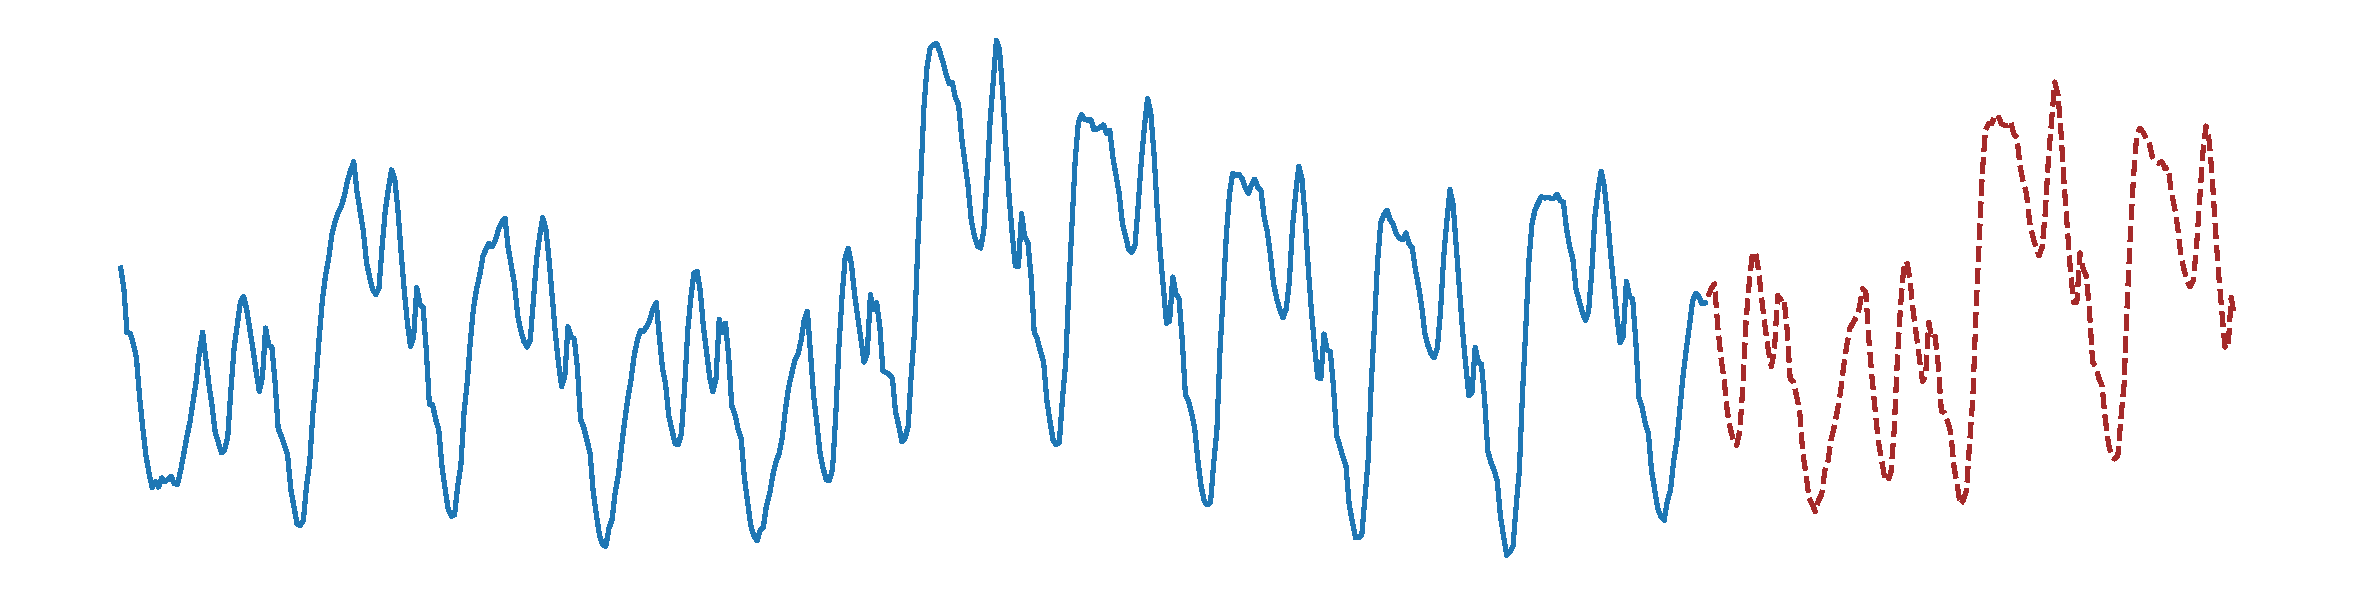
\includegraphics[width=0.58\linewidth]
    {Images/time-series/national-load-curves-forecast.pdf}

  \scriptsize Individual electricity load curve: observed lookback and
  horizon to forecast.
\end{frame}

\section{Current context}

\begin{frame}{Foundation Models (FMs)}
  \small
  \textbf{Foundation models}, such as \texttt{Chronos-2}, \texttt{TabPFN-TS}, and  \texttt{TS-ICL} \citep{chronos2,tabpfn-ts,ts-icl}, have become state-of-the-art in forecasting. Notable properties:
  \begin{itemize}
      \item Pretrained on huge datasets mixing real-world and synthetic time series (large \textbf{prior}).
      \item Perform gradient-free \textbf{in-context learning}
      \item Modern architectures take optional \textbf{covariates} as inputs:
        \[
        \hat y = f_\theta(x,z) \in\mathbb{R}^{L+H}
        \]
      \end{itemize}

  \medskip

\begin{figure}
    \centering
    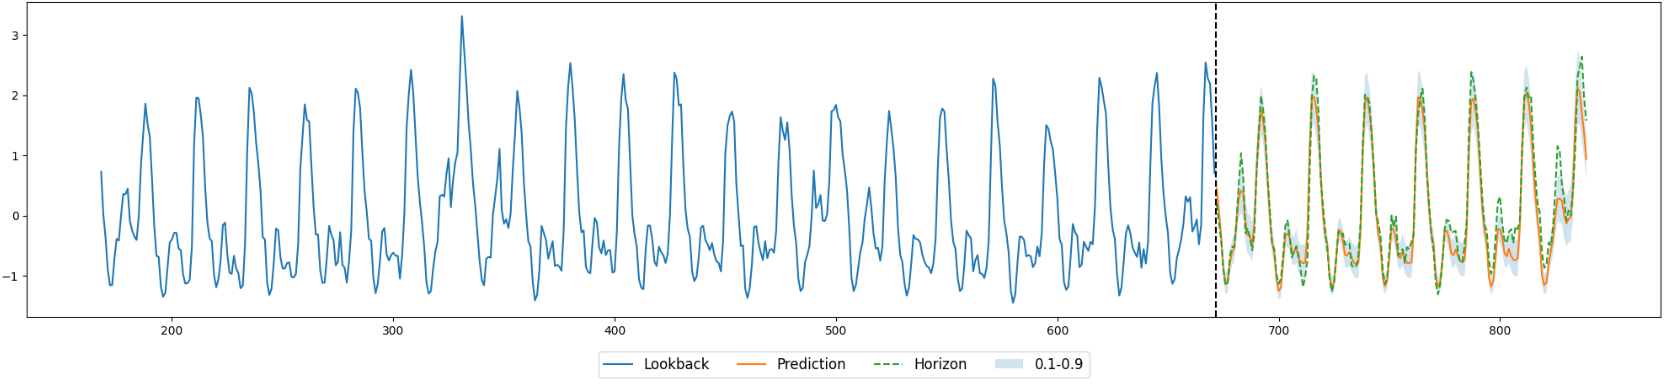
\includegraphics[width=0.8\linewidth]{Images/ongoing/chronos_prev.png}
    \vspace{-3mm}
    \caption{Example prediction of \texttt{Chronos-2} on \textsc{Electricity}}
    \label{fig:placeholder}
\end{figure}
  
\end{frame}

\begin{frame}{How to Adapt to Local Context?}

    \begin{figure}
        \centering
        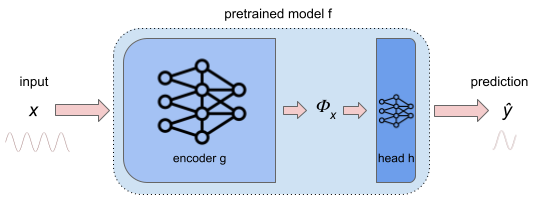
\includegraphics[width=0.4\linewidth]{Images/ongoing/pretrained-model.png}
        \caption{Illustration of a pretrained forecasting model. Models such as \texttt{Chronos-2} (120M parameters) are composed of multiple temporal and cross-variate attention layers. }
        \label{fig:placeholder}
    \end{figure}

  \small
  \begin{itemize}
    \item \textbf{Fine-tuning}: update part or all of the pretrained model on
      local data.
    \item \textbf{LoRA}: learn low-rank adaptation weights while keeping most
      pretrained parameters fixed.
    \item \textbf{Adding covariates}: adding \textit{relevant} covariates to the inputs.

    Promising direction to adapt locally \textit{without intensive tuning}
  \end{itemize}

\end{frame}

\begin{frame}{Adding covariates is not trivial}

Assume $Y_t = f^*(t,Z_t)=a+bt+Z_t$ with $Z_t = ct$.

\begin{itemize}
    \item Optimal linear model on $t$ is $Y_t = f_0(t) = a+(b+c)t $
    \item One possible model over $t$ and $Z_t$ is $Y_t = f_2(t,Z_t) = a+ 0.t+\frac{b+c}{c}Z_t$
\end{itemize}

Now if $Z_t \sim Z_{t-1}+\epsilon_t$, its information is crucial.

This examples shows adding information can both be necessary or detrimental (even when causally relevant).

\ColorBox{edf1}{}{Finding \textit{relevant} covariates for prediction is essential. But what is relevant? In our setting, we only have access to one's own past data, and other users' past data.}

\end{frame}

\begin{frame}{Adding covariates is not trivial}

\only<1>{
\begin{figure}
    \centering
    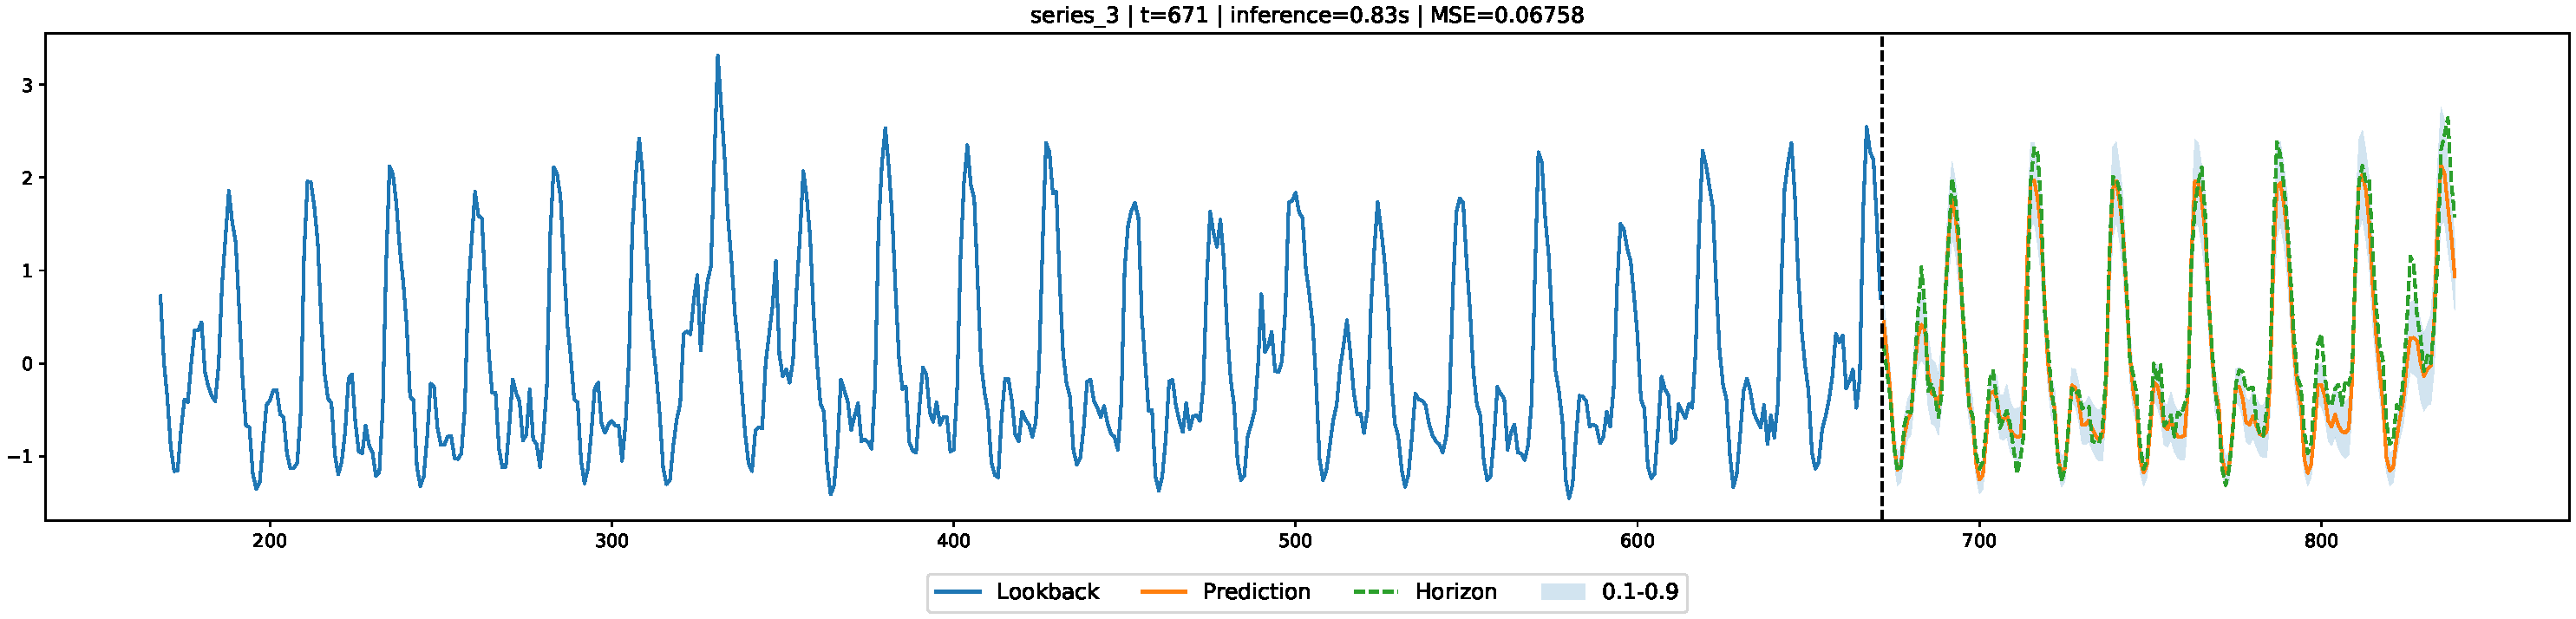
\includegraphics[width=\linewidth]{Images/ongoing/chronos_forecast_series_3_t671_lag672_h168.pdf}
    \caption{Example \textit{univariate} prediction, MSE=0.068}
    \label{fig:placeholder}
\end{figure}
}


\only<2>{
\begin{figure}
    \centering
    \includegraphics[width=\linewidth]{Images/ongoing/chronos_forecast_series_3_t671_lag672_h168 (4).pdf}
    \caption{Example prediction with covariate, MSE=0.2293}
    \label{fig:placeholder}
\end{figure}
}

\only<3>{
\begin{figure}
    \centering
    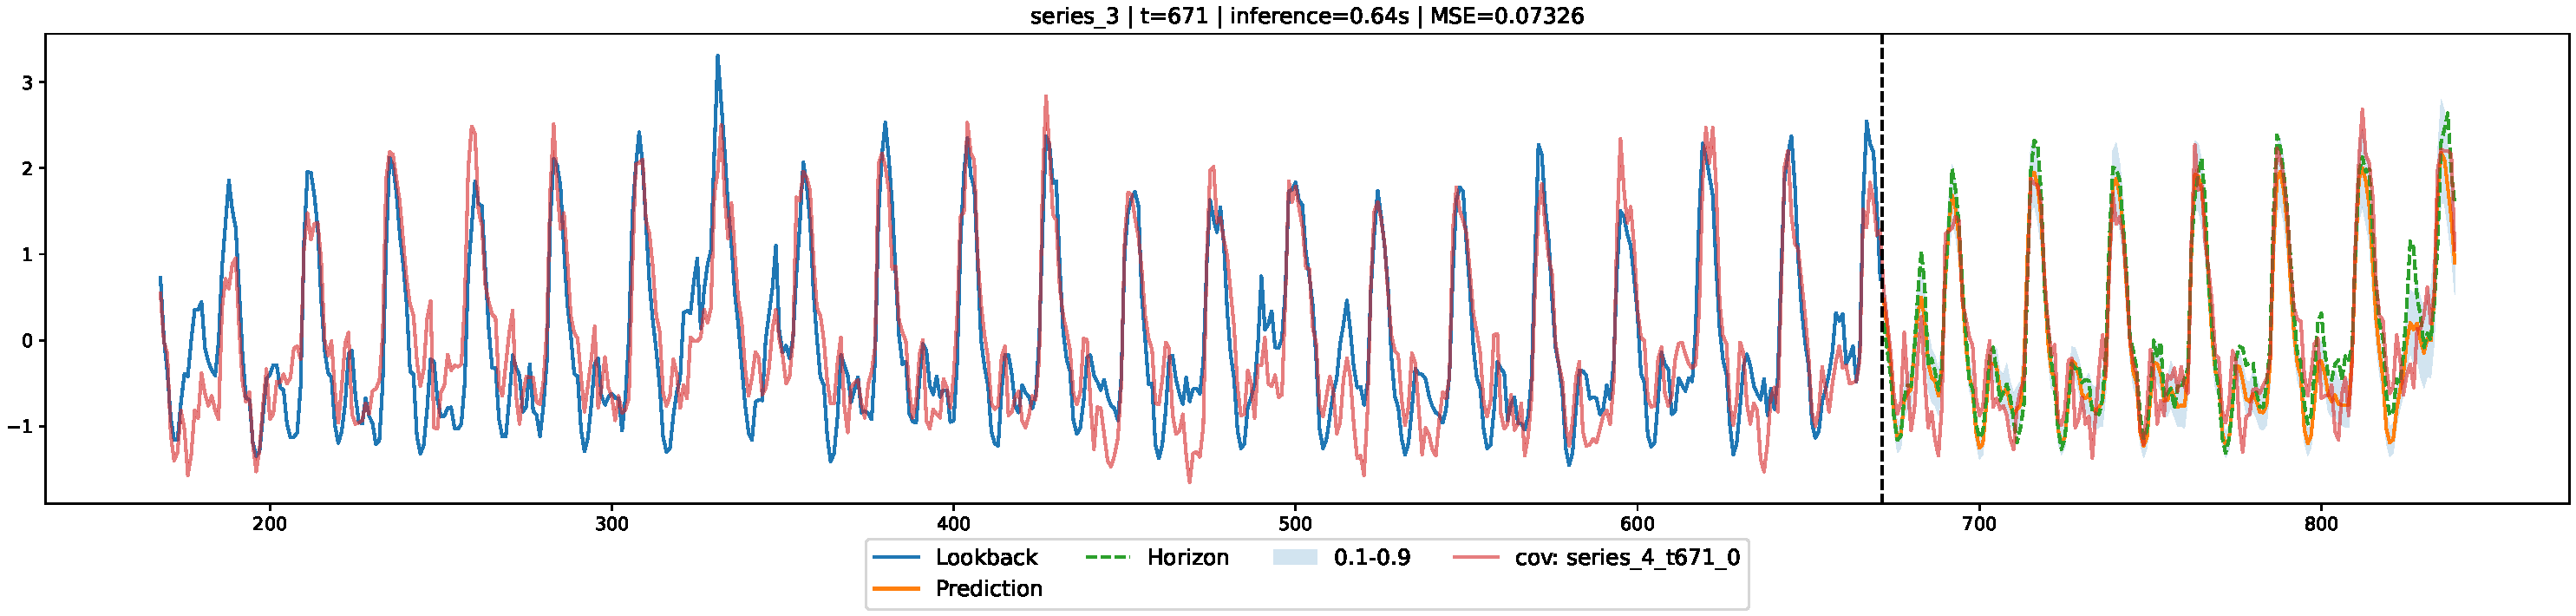
\includegraphics[width=\linewidth]{Images/ongoing/chronos_forecast_series_3_t671_lag672_h168 (2).pdf}
    \caption{Example prediction with covariate, MSE=0.0733}
    \label{fig:placeholder}
\end{figure}
}

\end{frame}

\begin{frame}{Adding covariates is not trivial}

\ColorBox{edf4}{}{
\begin{itemize}

\item Current FMs do not detect easy causal cross-variate patterns very well, even if all information is provided in context  \citep{berthelierinvestigating}
    
\item We tested adding closest windows as covariates: on average, it degrades performance.

\end{itemize}
}

\ColorBox{edf1}{}{
\begin{itemize}
    
% \item Adding transformations of the inputs (e.g sign and square-root) slightly improves performance.
%on verra plus tard pour cet ajout

\item On roughly 50\% of windows, closest windows do improve performance.\\{\color{blue} With optimal decision, can achieve 10\% improvement!}

\end{itemize}
}

Idea: learn a gate that decides when to use $\hat{y}=f(x)$ or $\hat{y}^c=f(x,z)$.

\end{frame}

\begin{frame}{Gated conditioned prediction}

We'd want to train a model:
\[ \hat y_{\mathrm{adapted}} = \sigma(\hat{y},\hat{y}^c) \]

\[ \hat y_{\mathrm{adapted}} = \sigma(x,X_c, \hat{y},\hat{y}^c) \]

\begin{itemize}
    \item No-feature Bayes gates learn only a scalar or horizon-wise decision from T2.
    \item CatBoost gates use retrieval and forecast features to make instance-specific decisions.
\end{itemize}

    
\end{frame}


\begin{frame}{Retrieval-Augmented Generation (RAG)}
  \begin{columns}[T,onlytextwidth]
    \begin{column}{0.48\textwidth}
      \small
      For a target lookback window $x$, retrieve aligned historical neighbors from the local datastore:
\[
\mathcal{N}(x)=\{(x_k,y_k)\}_{k=1}^{K}, \qquad
x_k \approx x.
\]

This allows to compute the context-conditioned forecast $\hat y^c= f(x, \mathcal{N}(x))$.

\medskip
\underline{But it also gives us past ground-truths $\{y_k\}_{k=1}^K$}
    \end{column}
    \begin{column}{0.48\textwidth}
      \centering
      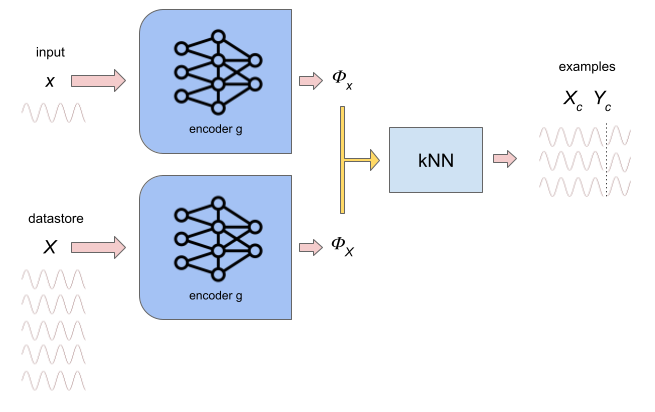
\includegraphics[width=0.92\linewidth]
        {Images/ongoing/neighbors.png}

      \scriptsize k-NN retrieval of aligned historical examples.
    \end{column}
  \end{columns}
\end{frame}

\begin{frame}{Fetching neighbors}

    \begin{itemize}
    
    \item Fitting a convex combination of outputs with local datastore is beneficial in NLP tasks \citep{khandelwal2019generalization,marfoq2022personalized}.

    \item Recent models such as Cross-RAG \citep{lee2026cross} fuse retrieved examples' \textit{latent representations} with the query, to decode a new forecast.

    \end{itemize}

\ColorBox{edf2}{}{It is possible to learn to fuse information from neighbors to improve prediction!}

\begin{figure}
        \centering
        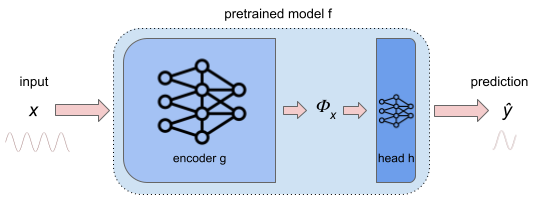
\includegraphics[width=0.4\linewidth]{Images/ongoing/pretrained-model.png}
        \label{fig:placeholder}
    \end{figure}

\end{frame}


\section{Proposal}

\begin{frame}{Retrieval-Based Residual Adaptation}
  \begin{columns}[T,onlytextwidth]
    \begin{column}{0.48\textwidth}
      \small
      The adapter receives four complementary signals:
      \begin{itemize}
        \item the vanilla forecast $\hat y$;
        \item the context-conditioned forecast $\hat y^c$;
        \item realized horizons $Y_c$ from similar examples;
        \item local residuals $R_c=Y_c-\hat Y_c$.
      \end{itemize}

      \medskip
      The goal is to improve $\hat y$ while keeping the correction lightweight,
      interpretable, and conservative.
    \end{column}
    \begin{column}{0.48\textwidth}
      \centering
      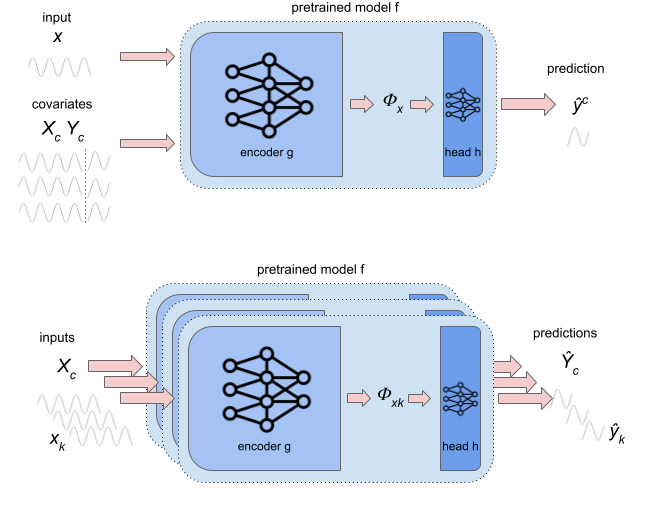
\includegraphics[width=\linewidth]
        {Images/ongoing/predictions.png}

      \scriptsize Extra predictions expose both memory and model errors.
    \end{column}
  \end{columns}
\end{frame}

\begin{frame}{Baseline Adapters}
  \small
  Before introducing a deeper adapter, compare against simple output-space
  corrections:

  \begin{table}
    \centering
    \begin{tabular}{lll}
      \toprule
      \textbf{Adapter} & \textbf{Signal used} & \textbf{Trainable part} \\
      \midrule
      Gate on conditioned-prediction & $\hat y, \hat y^c$ & scalar or horizon-wise decisions \\
      Weighted mix of horizons & $\hat y, Y_c$ & fixed via distance, learned convex or ridge  \\
      Weighted residual  & $\hat y, R_c$ & fixed via distance, learned convex or ridge\\
      Full mixture & $\hat y, \hat y^c, Y_c$ & scalar or per-horizon \\
      \bottomrule
    \end{tabular}
  \end{table}

Example formulation of fixed mixture with one learned coefficient:
  \[
    \hat y_{\mathrm{mix}}
    =
    (1-\lambda)\hat y
    +
    \lambda\sum_{k=1}^{K} w_k y_k,
    \qquad
    w_k =
    \frac{\exp(-d_k)}{\sum_{j=1}^{K}\exp(-d_j)}.
  \]
\end{frame}

\begin{frame}{Baseline Sweep Results}
  \tiny
  \centering
  \begin{tabular}{lrrrrrr}
    \toprule
    \textbf{Electricity 168--24} &
    \textbf{raw-1} & \textbf{raw-3} & \textbf{raw-10} &
    \textbf{IN-1} & \textbf{IN-3} & \textbf{IN-10} \\
    \midrule
    Context forecast $\hat y^c$ & -- & -- & -- & -- & -- & -- \\
    Horizon kNN, weighted & -- & -- & -- & -- & -- & -- \\
    Horizon scalar mix & -- & -- & -- & -- & -- & -- \\
    Horizon ridge, shared & -- & -- & -- & -- & -- & -- \\
    Residual kNN, weighted & -- & -- & -- & -- & -- & -- \\
    Residual scalar mix & -- & -- & -- & -- & -- & -- \\
    Residual ridge, shared & -- & -- & -- & -- & -- & -- \\
    Residual ridge, horizon & -- & -- & -- & -- & -- & -- \\
    Full ridge, horizon & -- & -- & -- & -- & -- & -- \\
    \bottomrule
  \end{tabular}

  \vspace{0.25cm}
  \scriptsize nMSE on T3. Lower is better.
\end{frame}

\begin{frame}{Gate Sweep Results}
  \tiny
  \centering
  \begin{tabular}{lrrrrrr}
    \toprule
    \textbf{Electricity 168--24} &
    \textbf{raw-1} & \textbf{raw-3} & \textbf{raw-10} &
    \textbf{IN-1} & \textbf{IN-3} & \textbf{IN-10} \\
    \midrule
    Bayes gate, scalar & -- & -- & -- & -- & -- & -- \\
    Bayes gate, horizon & -- & -- & -- & -- & -- & -- \\
    CatBoost classifier, scalar & -- & -- & -- & -- & -- & -- \\
    CatBoost classifier, horizon & -- & -- & -- & -- & -- & -- \\
    CatBoost regressor, scalar & -- & -- & -- & -- & -- & -- \\
    CatBoost regressor, horizon & -- & -- & -- & -- & -- & -- \\
    Oracle, scalar & -- & -- & -- & -- & -- & -- \\
    Oracle, horizon & -- & -- & -- & -- & -- & -- \\
    \bottomrule
  \end{tabular}

  \vspace{0.25cm}
  \scriptsize Bayes gates use no features; CatBoost gates use the feature set in appendix.
\end{frame}

% \begin{frame}{Time-Series Informed Forecast Adapter (TS-IFA)}
%   \begin{columns}[T,onlytextwidth]
%     \begin{column}{0.62\textwidth}
%       \centering
%       \includegraphics[height=0.84\textheight]
%         {Images/ongoing/pipeline.png}
%     \end{column}
%     \begin{column}{0.36\textwidth}
%       \small
%       \begin{itemize}
%         \item A residual branch embeds local errors $R_c$ into $y_r$.
%         \item A memory branch embeds realized horizons $Y_c$ into $y_m$.
%         \item A final attention layer mixes $\hat y$, $\hat y^c$, $y_r$, and
%           $y_m$ into $\hat y_{\mathrm{adapt}}$.
%       \end{itemize}

%       \footnotesize
%       Cross-attention makes each correction traceable to retrieved windows and
%       to one of the candidate forecasts.
%     \end{column}
%   \end{columns}
% \end{frame}

\begin{frame}{Residual and Memory Branches}
  \small
  Define joint input-prediction representations
  \[
    m=[x,\hat y],
    \qquad
    M_c=[X_c,\hat Y_c].
  \]

  \begin{columns}[T,onlytextwidth]
    \begin{column}{0.48\textwidth}
      \ColorBox{edf2}{Residual branch}{%
        \[
          z_r=\operatorname{Attn}(m,M_c,R_c),
          \qquad
          y_r=\hat y+\operatorname{MLP}(\hat{y}, z_r).
        \]
        $z_r$ asks how the frozen model was wrong in similar states.
      }
    \end{column}
    \begin{column}{0.48\textwidth}
      \ColorBox{edf6}{Memory branch}{%
        \[
          z_m=\operatorname{Attn}(x,X_c,Y_c),
          \qquad
          y_m=\hat{y}+\operatorname{MLP}([\hat y,z_m]).
        \]
        $z_m$ learns how much realized neighbor horizons inform on the forecast.
      }
    \end{column}
  \end{columns}
\end{frame}

\begin{frame}{Final Mixture and Training Loss}
  \small
  The final layer mixes the four candidate forecasts:
  \[
    \tilde{Y}=[\hat y,\hat y^c,y_r,y_m] \in \mathbb{R}^{4\times H},
    \qquad z=\operatorname{Attn}(x,X_c,X_c) \in \mathbb{R}^{1\times L}
  \]

  \[ \alpha = \operatorname{softmax}(\operatorname{MLP}(z)) \in \mathbb{R}^{4 \times H} \qquad 
    \hat y_{\mathrm{adapted}}
    = \alpha \odot \tilde{Y}=(\sum_{i=1}^4 \alpha_{i,h} \tilde{Y}_{i,h})_h
  \]

  
\end{frame}

\begin{frame}{TS-IFA Results}
  \scriptsize
  \centering
  \begin{tabular}{llrrrr}
    \toprule
    \textbf{Dataset} & \textbf{$L$--$H$} &
    \textbf{Chronos} & \textbf{Best baseline} &
    \textbf{Best gate} & \textbf{TS-IFA} \\
    \midrule
    Electricity & 168--24 & -- & -- & -- & -- \\
    Electricity & 672--168 & -- & -- & -- & -- \\
    Solar & 168--24 & -- & -- & -- & -- \\
    Solar & 672--168 & -- & -- & -- & -- \\
    \bottomrule
  \end{tabular}

  \vspace{0.25cm}
  \scriptsize nMSE on T3. Lower is better.
\end{frame}

\begin{frame}[standout]
  Thank you\\
  Questions?
\end{frame}

\appendix
\section{Appendix}

\begin{frame}{Appendix: Baseline Formulas}
  \scriptsize
  Let $r_k=y_k-\hat y_k$, and
  \[
    w_k=\frac{\exp(-d_k)}{\sum_j \exp(-d_j)}.
  \]

  Horizon baselines:
  \[
    \hat y_{\mathrm{Y\mbox{-}kNN}}=\sum_k w_k y_k,
    \qquad
    \hat y_{\mathrm{Y\mbox{-}mix}}=(1-\lambda)\hat y+\lambda\sum_k w_k y_k.
  \]
  \[
    \hat y_{\mathrm{Y\mbox{-}ridge}}=\hat y+
    \beta_0\hat y+\sum_k\beta_k y_k.
  \]

  Residual baselines:
  \[
    \hat y_{\mathrm{R\mbox{-}kNN}}=\hat y+\sum_k w_k r_k,
    \qquad
    \hat y_{\mathrm{R\mbox{-}mix}}=\hat y+\lambda\sum_k w_k r_k.
  \]
  \[
    \hat y_{\mathrm{R\mbox{-}ridge}}=\hat y+\sum_k\beta_k r_k,
    \qquad
    \hat y_{\mathrm{R\mbox{-}ridge},h}=\hat y_h+\sum_k \beta_{k,h} r_{k,h}.
  \]

  Full horizon-wise ridge:
  \[
    \hat y_{\mathrm{full},h}
    =\hat y_h+\beta_{0,h}\hat y_h+\beta_{c,h}\hat y^c_h
     +\sum_k\beta_{k,h}y_{k,h}.
  \]
\end{frame}

\begin{frame}{Appendix: Gate Features}
  \scriptsize
  Gate targets compare vanilla and context-conditioned losses:
  \[
    \Delta_h=(y_h-\hat y_h)^2-(y_h-\hat y^c_h)^2.
  \]

  \begin{columns}[T,onlytextwidth]
    \begin{column}{0.48\textwidth}
      \textbf{Decision shapes}
      \begin{itemize}
        \item scalar: target $\frac{1}{H}\sum_h\Delta_h$;
        \item horizon: targets $(\Delta_h)_{h=1}^H$.
      \end{itemize}

      \textbf{No-feature gates}
      \begin{itemize}
        \item Bayes-s: use context if $\mathbb{E}_{T2}[\Delta]>0$.
        \item Bayes-h: use context if $\mathbb{E}_{T2}[\Delta_h]>0$.
      \end{itemize}
    \end{column}
    \begin{column}{0.50\textwidth}
      \textbf{CatBoost features}
      \begin{itemize}
        \item context minus vanilla: mean/std or full horizon vector;
        \item weighted horizon minus vanilla mean;
        \item weighted residual mean;
        \item query mean and std;
        \item neighbor lookback mean: mean/std;
        \item neighbor lookback std: mean/std;
        \item same-user ratio and mean neighbor age;
        \item neighbor weight std/max;
        \item mean retrieval distance.
      \end{itemize}
    \end{column}
  \end{columns}
\end{frame}

\PrintBibliography


\end{document}
